\documentclass[12pt,titlepage]{article}
\usepackage[margin=1.25in]{geometry}
\usepackage{graphicx,amsmath,blindtext,enumitem}
\usepackage{tikz,tikz-qtree}
\usetikzlibrary{trees}

%% Variables definition
\newcommand{\vSubject}{Critical Thinking and Problem Solving}
\newcommand{\vSubtitle}{Critical Reasoning}
\newcommand{\vName}{Dicha Zelianivan Arkana}
\newcommand{\vNIM}{2241720002}
\newcommand{\vClass}{1i}
\newcommand{\vDepartment}{Information Technology}
\newcommand{\vStudyProgram}{D4 Informatics Engineering}

%% [START] Tikz related stuff
\usepackage{tikz}
\usetikzlibrary{svg.path,calc,shapes.geometric,shapes.misc}
\tikzstyle{terminator} = [rectangle, draw, text centered, rounded corners = 1em, minimum height=2em]
\tikzstyle{preparation} = [chamfered rectangle, chamfered rectangle sep=0.75em, draw, text centered, minimum height = 2em]
\tikzstyle{process} = [rectangle, draw, text centered, minimum height=2em]
\tikzstyle{decision} = [diamond, aspect=2, draw, text centered, minimum height=2em]
\tikzstyle{data}=[trapezium, draw, text centered, trapezium left angle=60, trapezium right angle=120, minimum height=2em]
\tikzstyle{connector} = [line width=0.25mm,->]
\tikzstyle{endpoint} = [isosceles triangle, isosceles triangle apex angle=60, anchor=apex, rotate=180, draw]
%% [END] Tikz related stuff

%% [START] Fancy header related stuff
\usepackage{fancyhdr}
\pagestyle{fancy}
\setlength{\headheight}{15pt} % compensate fancyhdr style
\fancyhead{}
\fancyfoot{}
\fancyfoot[L]{\thepage}
\fancyfoot[R]{\textit{\vSubject - \vSubtitle}}
\renewcommand{\footrulewidth}{0.4pt}% default is 0pt, overline for footer
%% [END] Fancy header related stuff

%% [START] Custom tabular command related stuff
\usepackage{tabularx}
\newcommand{\details}[2]{
    #1 & #2  \\
}
%% [END] Custom tabular command related stuff

%% [START] Figure related stuff
\newcommand{\image}[3][1]{
    \begin{figure}[h]
        \centering
        \includegraphics[#1]{#2}
        \caption{#3}
        \label{#3}
    \end{figure}
}
%% [END] Figure related stuff

\begin{document}
\begin{titlepage}
    \centering
    \vfill
    {\bfseries\LARGE
        \vSubject\\
        \vskip0.25cm
        \vSubtitle
    }
    \vfill
    
\includegraphics[width=6cm]{images/polinema-logo.png}
    \vfill
    {
        \textbf{Name}\\
        \vName\\
        \vskip0.5cm
        \textbf{NIM}\\
        \vNIM\\
        \vskip0.5cm
        \textbf{Class}\\
        \vClass\\
        \vskip0.5cm
        \textbf{Department}\\
        \vDepartment\\
        \vskip0.5cm
        \textbf{Study Program}\\
        \vStudyProgram
    }
\end{titlepage}

\section{Task}
Suppose a new team of analysts has reassessed a shale gas deposit based on new evidence and technological improvements. Extraction costs remain the same, but the team now estimates that there are:
\begin{itemize}
    \item No harm from level C (returns \$2 million)
    \item Only 30\% chance of a level B result (\$7 million return)
    \item 40\% chance of a level A returns (\$12 million return)
    \item 25\% chance of getting level AA results (\$24 million return)
    \item 5\% chance of AAA level results (\$40 million return)
\end{itemize}
A rival company called YGN has bid \$10 million for the extraction rights.
Calculate possible new returns, using a decision tree if that helps you. Then decide which of the following can most reliably be inferred from the data.
\begin{enumerate}[label=\Alph*.)]
    \item On economic grounds alone, the Zenergies should accept YGN's offer
    \item On economic grounds alone, the Zenergies should decline Yangen's offer and continue extraction
    \item It makes no difference economically which decision the Zenergies make.
\end{enumerate}

\pagebreak

\subsection*{Step 1 - Drawing Branches}

There are 3 statements that is possible, but there is only one that is most suitable for this situation.
First up, the extraction cost is \$3 million, so we need to keep that into account when we count the profit.

There are 2 paths, though. The first one, a bit risky, but the reward could bemuch higher than the second option,
which is we play it safe by selling it to YGN and earn a fixed amount up front.

Also, we need to pay the amount of the extraction cost up front if we go with the first route.


\begin{center}
    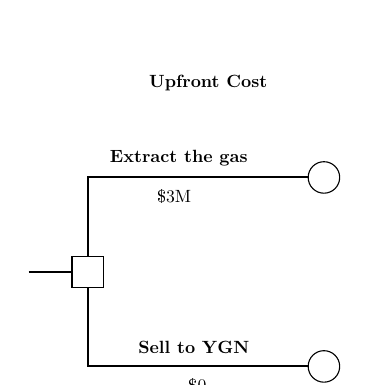
\begin{tikzpicture}[every node/.style={scale=0.8}]
        \node (root) [rectangle, draw, minimum width=5mm, minimum height=5mm] {};
        \node (branch-1) [circle, draw, right of=root, xshift=2.75cm, yshift=1.5cm, minimum width=5mm, minimum height=5mm] {};
        \node (branch-2) [circle, draw, right of=root, xshift=2.75cm, yshift=-1.5cm, minimum width=5mm, minimum height=5mm] {};
        \node (label-1) [above of=branch-1,left=8mm,yshift=5mm,scale=0.8] {\textbf{Upfront Cost}};
        \draw [connector,-] (-7.5mm,0) -- (root.west);
        \draw [connector,-] (root.north) |- node[above=3mm,right=2.5mm,scale=0.8] {\textbf{Extract the gas}} 
                                            node[below=3mm,right=1cm,scale=0.8] {\$3M}
                            (branch-1.west);
        \draw [connector,-] (root.south) |- node[above=3mm,right=7mm,scale=0.8] {\textbf{Sell to YGN}}
                                            node[below=3mm,right=1.5cm,scale=0.8] {\$0}
                            (branch-2.west);
    \end{tikzpicture}
\end{center}


\subsection*{Step 2 - Drawing every possible cases}
After knowing those 2 paths, we need to draw every possible branches from them so we can visualise it better.
We should also write the profit, average profit, and overall profit to compare it later.

\begin{center}
    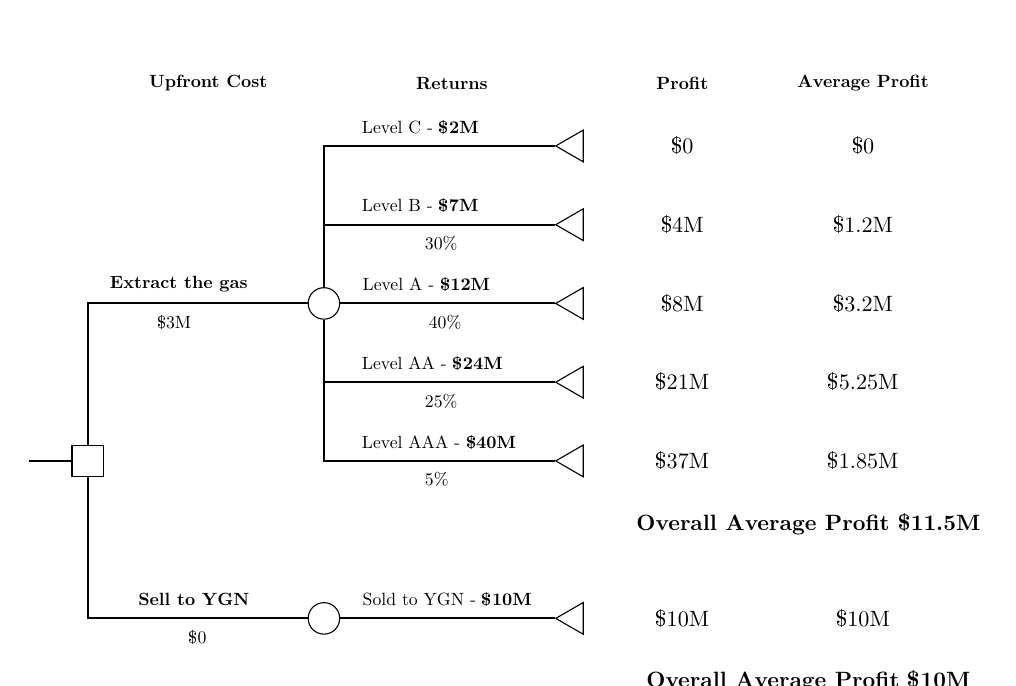
\begin{tikzpicture}[every node/.style={scale=0.8}]
        \node (root) [rectangle, draw, minimum width=5mm, minimum height=5mm] {};
        \node (branch-1) [circle, draw, right of=root, xshift=2.75cm, yshift=2.5cm, minimum width=5mm, minimum height=5mm] {};
        \node (branch-2) [circle, draw, right of=root, xshift=2.75cm, yshift=-2.5cm, minimum width=5mm, minimum height=5mm] {};
        \node (endpoint-1) [endpoint, right of = branch-1, xshift=-5cm, yshift=-2.5cm, minimum width=2.5mm, minimum height=2.5mm] {};
        \node (endpoint-2) [endpoint, right of = branch-1, xshift=-5cm, yshift=-1.25cm, minimum width=2.5mm, minimum height=2.5mm] {};
        \node (endpoint-3) [endpoint, right of = branch-1, xshift=-5cm, minimum width=2.5mm, minimum height=2.5mm] {};
        \node (endpoint-4) [endpoint, right of = branch-1, xshift=-5cm, yshift=1.25cm, minimum width=2.5mm, minimum height=2.5mm] {};
        \node (endpoint-5) [endpoint, right of = branch-1, xshift=-5cm, yshift=2.5cm, minimum width=2.5mm, minimum height=2.5mm] {};
        \node (endpoint-6) [endpoint, right of = branch-2, xshift=-5cm, minimum width=2.5mm, minimum height=2.5mm] {};
        \node (label-1) [above of=branch-1,left=8mm,yshift=2.5cm,scale=0.8] {\textbf{Upfront Cost}};
        \node (label-2) [above of=branch-1,left=8mm,yshift=2.5cm,xshift=3.5cm,scale=0.8] {\textbf{Returns}};
        \node (label-3) [above of=branch-1,left=8mm,yshift=2.5cm,xshift=7cm,scale=0.8] {\textbf{Profit}};
        \node (label-4) [above of=branch-1,left=8mm,yshift=2.5cm,xshift=10.5cm,scale=0.8] {\textbf{Average Profit}};
        \node (profit-1) [below of=label-3] {\$0};
        \node (profit-2) [below of=label-3,yshift=-1.25cm] {\$4M};
        \node (profit-3) [below of=label-3,yshift=-2.5cm] {\$8M};
        \node (profit-4) [below of=label-3,yshift=-3.75cm] {\$21M};
        \node (profit-5) [below of=label-3,yshift=-5cm] {\$37M};
        \node (profit-6) [below of=label-3,yshift=-7.5cm] {\$10M};
        \node (avg-profit-1) [below of=label-4] {\$0};
        \node (avg-profit-2) [below of=label-4,yshift=-1.25cm] {\$1.2M};
        \node (avg-profit-3) [below of=label-4,yshift=-2.5cm] {\$3.2M};
        \node (avg-profit-4) [below of=label-4,yshift=-3.75cm] {\$5.25M};
        \node (avg-profit-5) [below of=label-4,yshift=-5cm] {\$1.85M};
        \node (avg-profit-6) [below of=label-4,yshift=-7.5cm] {\$10M};
        \node (overall-avg) [below of=profit-5,xshift=2cm] {\textbf{Overall Average Profit \$11.5M}};
        \node (overall-sold-avg) [below of=profit-6,xshift=2cm] {\textbf{Overall Average Profit \$10M}};
        \draw [connector,-] (-7.5mm,0) -- (root.west);
        \draw [connector,-] (root.north) |- node[above=3mm,right=2.5mm,scale=0.8] {\textbf{Extract the gas}} 
                                            node[below=3mm,right=1cm,scale=0.8] {\$3M}
                            (branch-1.west);
        \draw [connector,-] (root.south) |- node[above=3mm,right=7mm,scale=0.8] {\textbf{Sell to YGN}}
                                            node[below=3mm,right=1.5cm,scale=0.8] {\$0}
                            (branch-2.west);
        \draw [connector,-] (branch-1.north) |- node[above=3mm,right=5mm,scale=0.8] {Level C - \textbf{\$2M}} (endpoint-1);
        \draw [connector,-] (branch-1.north) |- node[above=3mm,right=5mm,scale=0.8] {Level B - \textbf{\$7M}} node[below=3mm,right=1.5cm,scale=0.8] {30\%} (endpoint-2);
        \draw [connector,-] (branch-1.east) -- node[above=3mm,right=-1.45cm,scale=0.8] {Level A - \textbf{\$12M}} node[below=3mm,right=-4mm,scale=0.8] {40\%} (endpoint-3);
        \draw [connector,-] (branch-1.south) |- node[above=3mm,right=5mm,scale=0.8] {Level AA - \textbf{\$24M}} node[below=3mm,right=1.5cm,scale=0.8] {25\%} (endpoint-4);
        \draw [connector,-] (branch-1.south) |- node[above=3mm,right=5mm,scale=0.8] {Level AAA - \textbf{\$40M}} node[below=3mm,right=1.5cm,scale=0.8] {5\%} (endpoint-5);
        \draw [connector,-] (branch-2.east) -- node[above=3mm,right=-1.45cm,scale=0.8] {Sold to YGN - \textbf{\$10M}} (endpoint-6);
    \end{tikzpicture}
\end{center}

\pagebreak

\subsection*{Step 3 - Reading the tree}
Based on our decision tree, we can see the overall average profit from both branches. The first one, if we decided to extract the gas
and take some risk, we have an overall average profit of \$11.5M. If we take the second one, we will get an overall average profit of \$10M.

From this information, we can say that the second statement, which says \textit{``On economic grounds alone, the Zenergies should decline Yangen's offer and continue extraction"}
is the most reliable statement because we can get \$1.5M more by extracting the gas rather than selling it to YGN.

\end{document}

